\documentclass[aspectratio=169, 11pt]{beamer}

% ── Theme & Colors ───────────────────────────────────────────
\usetheme{Madrid}
\usecolortheme{default}

\definecolor{tptblue}{RGB}{0, 62, 110}
\definecolor{tptlight}{RGB}{0, 120, 180}
\definecolor{tptgray}{RGB}{100, 100, 100}
\definecolor{okgreen}{RGB}{34, 139, 34}
\definecolor{warnor}{RGB}{200, 120, 0}

\setbeamercolor{structure}{fg=tptblue}
\setbeamercolor{frametitle}{bg=tptblue, fg=white}
\setbeamercolor{title}{fg=white, bg=tptblue}
\setbeamercolor{block title}{bg=tptblue, fg=white}
\setbeamercolor{block body}{bg=tptblue!5}
\setbeamercolor{item}{fg=tptblue}

\setbeamertemplate{navigation symbols}{}
\setbeamertemplate{footline}{%
  \leavevmode\hbox{%
    \begin{beamercolorbox}[wd=.33\paperwidth,ht=2.5ex,dp=1ex,center]{author in head/foot}%
      \usebeamerfont{author in head/foot}\insertshortauthor
    \end{beamercolorbox}%
    \begin{beamercolorbox}[wd=.34\paperwidth,ht=2.5ex,dp=1ex,center]{title in head/foot}%
      \usebeamerfont{title in head/foot}DATA713 --- MLOps
    \end{beamercolorbox}%
    \begin{beamercolorbox}[wd=.33\paperwidth,ht=2.5ex,dp=1ex,right]{date in head/foot}%
      \insertframenumber{} / \inserttotalframenumber\hspace*{2em}
    \end{beamercolorbox}}%
}

% ── Packages ─────────────────────────────────────────────────
\usepackage[utf8]{inputenc}
\usepackage[T1]{fontenc}
\usepackage{graphicx}
\usepackage{booktabs}
\usepackage{tabularx}
\usepackage{multicol}
\usepackage{tikz}
\usetikzlibrary{arrows.meta, positioning, shapes.geometric, fit, calc}
\usepackage{fontawesome5}
\usepackage{hyperref}

% ── Meta ─────────────────────────────────────────────────────
\title[Hydraulic Condition Monitoring]{Hydraulic System Condition Monitoring\\[4pt]\small MLOps Pipeline --- From Training to Production}
\author[Groupe MLOps]{Personne A \quad Personne B \quad Personne C \quad Personne D}
\institute{
\includegraphics[height=1cm]{logo_telecom_ipparis_rvb_fond_h-770x360.png}}
\date{DATA713 --- Mars 2026}

\begin{document}

% ═══════════════════════════════════════════════════════════════
% SLIDE 1 — Title
% ═══════════════════════════════════════════════════════════════
\begin{frame}[plain]
  \titlepage
\end{frame}

% ═══════════════════════════════════════════════════════════════
% SLIDE 2 — Context & Problem
% ═══════════════════════════════════════════════════════════════
\begin{frame}{Context \& Problem}

\begin{columns}[T]
  \begin{column}{0.55\textwidth}
    \textbf{Use case:} Industrial predictive maintenance\\[6pt]
    \textbf{Dataset:} UCI --- Condition Monitoring of Hydraulic Systems
    \begin{itemize}
      \item 2205 operating cycles $\times$ 17 sensors
      \item 4 component conditions to predict simultaneously
      \item Labels from \texttt{profile.txt} (supervised)
    \end{itemize}
    \vspace{8pt}
    \textbf{Formulation:} Multi-class multi-output classification\\
    {\small\color{tptgray} Not anomaly detection --- labeled data allows per-component diagnostics}
  \end{column}

  \begin{column}{0.42\textwidth}
    \small
    \begin{tabular}{@{}lll@{}}
      \toprule
      \textbf{Target} & \textbf{Component} & \textbf{Classes} \\
      \midrule
      cooler & Cooler & 3 \\
      valve & Valve & 4 \\
      pump & Pump & 3 \\
      accumulator & Accum. & 4 \\
      \bottomrule
    \end{tabular}
    \vspace{10pt}

    \textbf{17 sensors:}\\
    {\footnotesize PS1--PS6, EPS1, FS1--FS2,\\TS1--TS4, VS1, CE, CP, SE}\\[4pt]
    {\footnotesize Feature eng.: mean per cycle}
  \end{column}
\end{columns}

\end{frame}

% ═══════════════════════════════════════════════════════════════
% SLIDE 3 — Architecture Overview
% ═══════════════════════════════════════════════════════════════
\begin{frame}[fragile]{Architecture Overview}

\centering
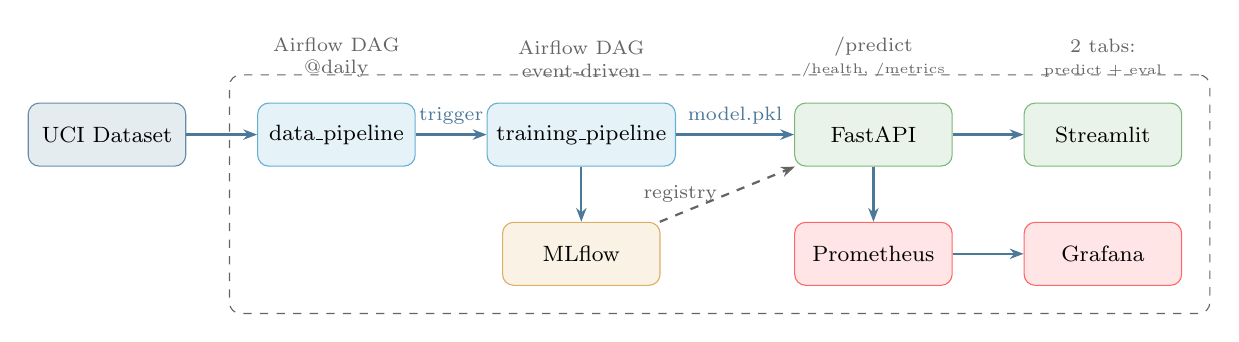
\begin{tikzpicture}[
    node distance=0.6cm and 0.9cm,
    box/.style={draw, rounded corners, minimum height=0.8cm, minimum width=2cm, font=\footnotesize, fill=#1!10, draw=#1!60},
    box/.default=tptblue,
    arrow/.style={-{Stealth[length=5pt]}, thick, tptblue!70},
    label/.style={font=\scriptsize\color{tptgray}, align=center},
  ]

  % Data layer
  \node[box=tptblue] (uci) {UCI Dataset};
  \node[box=tptlight, right=of uci] (datapipe) {data\_pipeline};
  \node[box=tptlight, right=of datapipe] (trainpipe) {training\_pipeline};

  % MLflow
  \node[box=warnor, below=0.7cm of trainpipe] (mlflow) {MLflow};

  % Serving layer
  \node[box=okgreen, right=1.5cm of trainpipe] (api) {FastAPI};
  \node[box=okgreen, right=of api] (webapp) {Streamlit};

  % Monitoring
  \node[box=red, below=0.7cm of api] (prom) {Prometheus};
  \node[box=red, right=of prom] (grafana) {Grafana};

  % Infra labels
  \node[label, above=0.2cm of datapipe] {Airflow DAG\\@daily};
  \node[label, above=0.2cm of trainpipe] {Airflow DAG\\event-driven};
  \node[label, above=0.2cm of api] {/predict\\{\tiny /health, /metrics}};
  \node[label, above=0.2cm of webapp] {2 tabs:\\{\tiny predict + eval}};

  % Arrows
  \draw[arrow] (uci) -- (datapipe);
  \draw[arrow] (datapipe) -- node[above, font=\scriptsize] {trigger} (trainpipe);
  \draw[arrow] (trainpipe) -- (mlflow);
  \draw[arrow] (trainpipe) -- node[above, font=\scriptsize] {model.pkl} (api);
  \draw[arrow] (api) -- (webapp);
  \draw[arrow] (api) -- (prom);
  \draw[arrow] (prom) -- (grafana);
  \draw[arrow, dashed, tptgray] (mlflow) -- node[left, font=\scriptsize, text=tptgray] {registry} (api);

  % Docker Compose box
  \node[draw=tptgray, dashed, rounded corners, fit=(datapipe)(trainpipe)(mlflow)(api)(webapp)(prom)(grafana),
        inner sep=10pt, label={[font=\scriptsize\color{tptgray}]below left:Docker Compose --- 9 services}] {};

\end{tikzpicture}

\vspace{4pt}
\begin{columns}[T]
  \begin{column}{0.48\textwidth}
    \footnotesize
    \textbf{Dev:} \texttt{docker compose up} (9 services)
  \end{column}
  \begin{column}{0.48\textwidth}
    \footnotesize
    \textbf{Prod:} K8s manifests ready, CD conditional
  \end{column}
\end{columns}

\end{frame}

% ═══════════════════════════════════════════════════════════════
% SLIDE 4 — ML Pipeline & Continuous Training
% ═══════════════════════════════════════════════════════════════
\begin{frame}{ML Pipeline \& Continuous Training}

\begin{columns}[T]
  \begin{column}{0.52\textwidth}
    \textbf{Model:} \texttt{MultiOutputClassifier(RF)}\\[4pt]

    \textbf{Results (test set 20\%):}\\[2pt]
    \small
    \begin{tabular}{@{}lccc@{}}
      \toprule
      \textbf{Target} & \textbf{Acc.} & \textbf{F1\textsubscript{macro}} & \textbf{F1\textsubscript{weighted}} \\
      \midrule
      Cooler     & 1.000 & 1.000 & 1.000 \\
      Valve      & 0.948 & 0.947 & 0.948 \\
      Pump       & 0.993 & 0.993 & 0.993 \\
      Accumulator & 0.990 & 0.990 & 0.990 \\
      \bottomrule
    \end{tabular}

    \vspace{8pt}
    \textbf{MLflow tracks:}
    \begin{itemize}\small
      \item Params, metrics per target, model artifact
      \item JSON report (confusion matrices)
      \item Model Registry: promote / reject / archive
    \end{itemize}
  \end{column}

  \begin{column}{0.45\textwidth}
    \textbf{CT Logic (2 DAGs):}\\[4pt]
    \footnotesize
    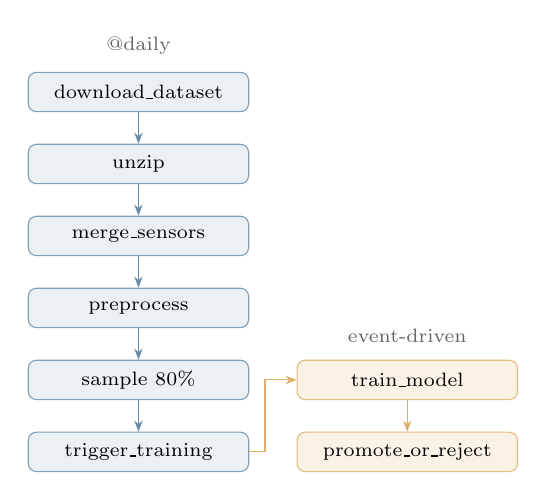
\begin{tikzpicture}[
      node distance=0.4cm,
      task/.style={draw, rounded corners=3pt, minimum width=2.8cm, minimum height=0.5cm, font=\scriptsize, fill=tptblue!8, draw=tptblue!50},
      arr/.style={-{Stealth[length=4pt]}, tptblue!60},
    ]
      \node[task] (dl) {download\_dataset};
      \node[task, below=of dl] (uz) {unzip};
      \node[task, below=of uz] (mg) {merge\_sensors};
      \node[task, below=of mg] (pp) {preprocess};
      \node[task, below=of pp] (sa) {sample 80\%};
      \node[task, below=of sa] (tr) {trigger\_training};

      \draw[arr] (dl)--(uz); \draw[arr] (uz)--(mg);
      \draw[arr] (mg)--(pp); \draw[arr] (pp)--(sa);
      \draw[arr] (sa)--(tr);

      \node[task, right=0.6cm of sa, fill=warnor!10, draw=warnor!50] (tm) {train\_model};
      \node[task, below=of tm, fill=warnor!10, draw=warnor!50] (pr) {promote\_or\_reject};

      \draw[arr, warnor!60] (tr.east) -- ++(0.2,0) |- (tm.west);
      \draw[arr, warnor!60] (tm)--(pr);

      \node[font=\scriptsize\color{tptgray}, above=0.1cm of dl] {@daily};
      \node[font=\scriptsize\color{tptgray}, above=0.1cm of tm] {event-driven};
    \end{tikzpicture}

    \vspace{6pt}
    {\scriptsize \textbf{Why 80\% sampling?} Static dataset --- sampling simulates data variability so champion/challenger comparison is meaningful.}
  \end{column}
\end{columns}

\end{frame}

% ═══════════════════════════════════════════════════════════════
% SLIDE 5 — CI/CD Pipeline
% ═══════════════════════════════════════════════════════════════
\begin{frame}[fragile]{CI/CD Pipeline}

\begin{columns}[T]
  \begin{column}{0.48\textwidth}
    \textbf{CI} {\small (every push \& PR)}\\[4pt]
    \begin{tikzpicture}[
      node distance=0.35cm,
      cibox/.style={draw, rounded corners=3pt, minimum width=3.5cm, minimum height=0.55cm, font=\small, fill=okgreen!8, draw=okgreen!50},
      arr/.style={-{Stealth[length=4pt]}, okgreen!60},
    ]
      \node[cibox] (lint) {\faCheck\hspace{4pt}ruff check};
      \node[cibox, below=of lint] (test) {\faCheck\hspace{4pt}pytest (26 tests)};
      \draw[arr] (lint)--(test);
    \end{tikzpicture}

    \vspace{8pt}
    \textbf{26 tests in 3 suites:}
    \small
    \begin{tabular}{@{}lr@{}}
      \toprule
      \textbf{Suite} & \textbf{Tests} \\
      \midrule
      DAG structure & 9 \\
      Model training & 7 \\
      Preprocessing & 10 \\
      \bottomrule
    \end{tabular}
  \end{column}

  \begin{column}{0.48\textwidth}
    \textbf{CD} {\small (push to main)}\\[4pt]
    \begin{tikzpicture}[
      node distance=0.35cm,
      cdbox/.style={draw, rounded corners=3pt, minimum width=3.8cm, minimum height=0.55cm, font=\small, fill=tptlight!10, draw=tptlight!50},
      arr/.style={-{Stealth[length=4pt]}, tptlight!60},
      skipbox/.style={draw, rounded corners=3pt, minimum width=3.8cm, minimum height=0.55cm, font=\small, fill=tptgray!10, draw=tptgray!40, text=tptgray},
    ]
      \node[cdbox] (test) {Run tests};
      \node[cdbox, below=of test] (build) {Build Docker images};
      \node[cdbox, below=of build] (push) {Push GHCR + DockerHub};
      \node[cdbox, below=of push] (check) {check-deploy (secrets?)};
      \node[skipbox, below=of check] (deploy) {\faForward\hspace{4pt}Deploy K8s (skipped)};
      \draw[arr] (test)--(build); \draw[arr] (build)--(push);
      \draw[arr] (push)--(check); \draw[arr, dashed, tptgray!60] (check)--(deploy);
    \end{tikzpicture}

    \vspace{4pt}
    {\scriptsize Tags: \texttt{latest} + git SHA (rollback)}\\
    {\scriptsize K8s deploy conditional on \texttt{KUBECONFIG} secret}
  \end{column}
\end{columns}

\end{frame}

% ═══════════════════════════════════════════════════════════════
% SLIDE 6 — API + WebApp + Monitoring
% ═══════════════════════════════════════════════════════════════
\begin{frame}{API, WebApp \& Monitoring}

\begin{columns}[T]
  \begin{column}{0.32\textwidth}
    \textbf{\faServer\hspace{4pt}FastAPI}\\[4pt]
    \small
    \begin{itemize}\setlength\itemsep{2pt}
      \item \texttt{POST /predict}\\{\scriptsize Pydantic body, 17 sensors $\to$ 4 states}
      \item \texttt{GET /health}\\{\scriptsize Readiness probe}
      \item \texttt{GET /metrics}\\{\scriptsize Prometheus instrumentation}
      \item \texttt{GET /docs}\\{\scriptsize Swagger auto-generated}
    \end{itemize}
  \end{column}

  \begin{column}{0.32\textwidth}
    \textbf{\faDesktop\hspace{4pt}Streamlit}\\[4pt]
    \small
    \textbf{Tab 1 --- Prediction}
    \begin{itemize}\setlength\itemsep{1pt}
      \item 17 sensor inputs
      \item Calls API $\to$ 4 predicted states
    \end{itemize}
    \vspace{4pt}
    \textbf{Tab 2 --- Model Evaluation}
    \begin{itemize}\setlength\itemsep{1pt}
      \item Accuracy, Precision, Recall, F1
      \item Confusion matrices
      \item Classification reports
    \end{itemize}
  \end{column}

  \begin{column}{0.32\textwidth}
    \textbf{\faChartBar\hspace{4pt}Monitoring}\\[4pt]
    \small
    \begin{itemize}\setlength\itemsep{2pt}
      \item \textbf{Prometheus}\\{\scriptsize Scrapes API \texttt{/metrics}\\+ Node Exporter}
      \item \textbf{Grafana}\\{\scriptsize Dashboard auto-provisioned\\on \texttt{docker compose up}}
      \item \textbf{Alerting}\\{\scriptsize Airflow email callbacks\\on DAG failure}
    \end{itemize}
  \end{column}
\end{columns}

\vspace{8pt}
\centering
{\small\color{tptgray} \faInfoCircle\hspace{4pt} Screenshots of each component available --- see backup slides}

\end{frame}

% ═══════════════════════════════════════════════════════════════
% SLIDE 7 — Collaboration & Lessons Learned
% ═══════════════════════════════════════════════════════════════
\begin{frame}{Collaboration \& Lessons Learned}

\begin{columns}[T]
  \begin{column}{0.48\textwidth}
    \textbf{Team organization:}\\[4pt]
    \small
    \begin{tabular}{@{}cp{5.5cm}@{}}
      \toprule
      & \textbf{Scope} \\
      \midrule
      A & Data \& ML pipeline, MLflow integration \\
      B & Airflow DAGs, CT, CI/CD, 26 tests, docs \\
      C & FastAPI API, Streamlit webapp \\
      D & Docker Compose, K8s, CD, monitoring \\
      \bottomrule
    \end{tabular}

    \vspace{8pt}
    \textbf{Git workflow:}
    \begin{itemize}\small
      \item Feature branches $\to$ PR $\to$ main
      \item CI gates (ruff + pytest)
      \item 20+ PRs, conventional commits
    \end{itemize}
  \end{column}

  \begin{column}{0.48\textwidth}
    \textbf{Honest limitations:}
    \begin{itemize}\small\setlength\itemsep{3pt}
      \item Dataset is static --- CT designed for production but trained on sampled data
      \item No K8s cluster --- CD pipeline ready, deploy step skipped
      \item API loads \texttt{model.pkl} locally, not from MLflow Registry
      \item Heavy Airflow imports --- learned to defer inside task functions
    \end{itemize}

    \vspace{6pt}
    \textbf{Key learning:}\\
    {\small Separation of concerns --- DAGs orchestrate, \texttt{src/} owns business logic, API serves, webapp displays.}
  \end{column}
\end{columns}

\end{frame}

% ═══════════════════════════════════════════════════════════════
% SLIDE 8 — Objectives Coverage
% ═══════════════════════════════════════════════════════════════
\begin{frame}{Objectives Coverage}

\small
\begin{columns}[T]
  \begin{column}{0.55\textwidth}
    \textbf{10/10 required objectives:}\\[3pt]
    \scriptsize
    \begin{tabular}{@{}clc@{}}
      \toprule
      \# & \textbf{Objective} & \textbf{Status} \\
      \midrule
      1 & Data extraction \& preprocessing & \textcolor{okgreen}{\faCheckCircle} \\
      2 & ML model & \textcolor{okgreen}{\faCheckCircle} \\
      3 & Model registry (MLflow) & \textcolor{okgreen}{\faCheckCircle} \\
      4 & Airflow retraining pipeline & \textcolor{okgreen}{\faCheckCircle} \\
      5 & MLflow experiment tracking & \textcolor{okgreen}{\faCheckCircle} \\
      6 & API (FastAPI + Swagger) & \textcolor{okgreen}{\faCheckCircle} \\
      7 & WebApp (Streamlit, 2 tabs) & \textcolor{okgreen}{\faCheckCircle} \\
      8 & Continuous Training (CT) & \textcolor{okgreen}{\faCheckCircle} \\
      9 & Docker + K8s + CI/CD & \textcolor{okgreen}{\faCheckCircle} \\
      10 & GitHub versioning \& docs & \textcolor{okgreen}{\faCheckCircle} \\
      \bottomrule
    \end{tabular}
  \end{column}

  \begin{column}{0.42\textwidth}
    \textbf{Bonus realized (3/8):}\\[3pt]
    \scriptsize
    \begin{tabular}{@{}clc@{}}
      \toprule
      \# & \textbf{Bonus} & \\
      \midrule
      12 & Monitoring (Prom+Grafana) & \textcolor{okgreen}{\faCheckCircle} \\
      14 & Model versioning/rollback & \textcolor{okgreen}{\faCheckCircle} \\
      17 & Email alerting & \textcolor{okgreen}{\faCheckCircle} \\
      \midrule
      11 & Live data & \textcolor{tptgray}{\faTimesCircle} \\
      13 & Load testing (Locust) & \textcolor{tptgray}{\faTimesCircle} \\
      15 & Human in the loop & \textcolor{tptgray}{\faTimesCircle} \\
      16 & API access mgmt & \textcolor{tptgray}{\faTimesCircle} \\
      \bottomrule
    \end{tabular}

    \vspace{10pt}
    \textbf{Stack:}\\[2pt]
    {\scriptsize Python 3.11 $\cdot$ scikit-learn $\cdot$ MLflow\\
    Airflow $\cdot$ FastAPI $\cdot$ Streamlit\\
    Docker $\cdot$ K8s $\cdot$ GitHub Actions\\
    Prometheus $\cdot$ Grafana $\cdot$ uv}
  \end{column}
\end{columns}

\end{frame}

% ═══════════════════════════════════════════════════════════════
% BACKUP — Screenshots placeholder
% ═══════════════════════════════════════════════════════════════
\appendix

\begin{frame}{Backup --- Screenshots}
  \centering
  \Large\color{tptgray}
  Screenshots to be added after\\
  \texttt{docker compose up} validation\\[12pt]
  \normalsize
  \begin{itemize}\color{tptgray}
    \item Airflow UI (both DAGs, task graph)
    \item MLflow UI (experiment runs, metrics)
    \item Swagger \texttt{/docs} (Pydantic schema)
    \item Streamlit Tab 1 (prediction) + Tab 2 (evaluation)
    \item Grafana dashboard
    \item GitHub Actions (CI green, CD pipeline)
    \item GitHub PRs with reviews
  \end{itemize}
\end{frame}

\end{document}
